\documentclass[a4paper, ngerman, 12pt,parskip=half]{scrreprt}
\usepackage{babel} % für Silbentrennung, eingedeutschte Verzeichnisnamen, etc.
\usepackage[utf8]{inputenc} % UTF8 Encoding
\usepackage[T1]{fontenc}  % Lateinisches Alphabet (T2 für Russisch, etc.)
\usepackage{booktabs} % für schöne Tabellen, siehe Termin 1
\usepackage{blindtext}
\usepackage{graphicx}
\usepackage{microtype} % Mikrotypografie, mit optischem Randausgleich

\begin{document}

\begin{titlepage}
{\large\textbf{Fernuni Hagen \\ 12345 Hagen \\ Lehrstuhl für Angew. Wissenschaften}}

\vspace*{4cm}

{\bfseries\huge Python und Perl im Vergleich -- Warum Python immer gewinnt! }

\begin{center}
	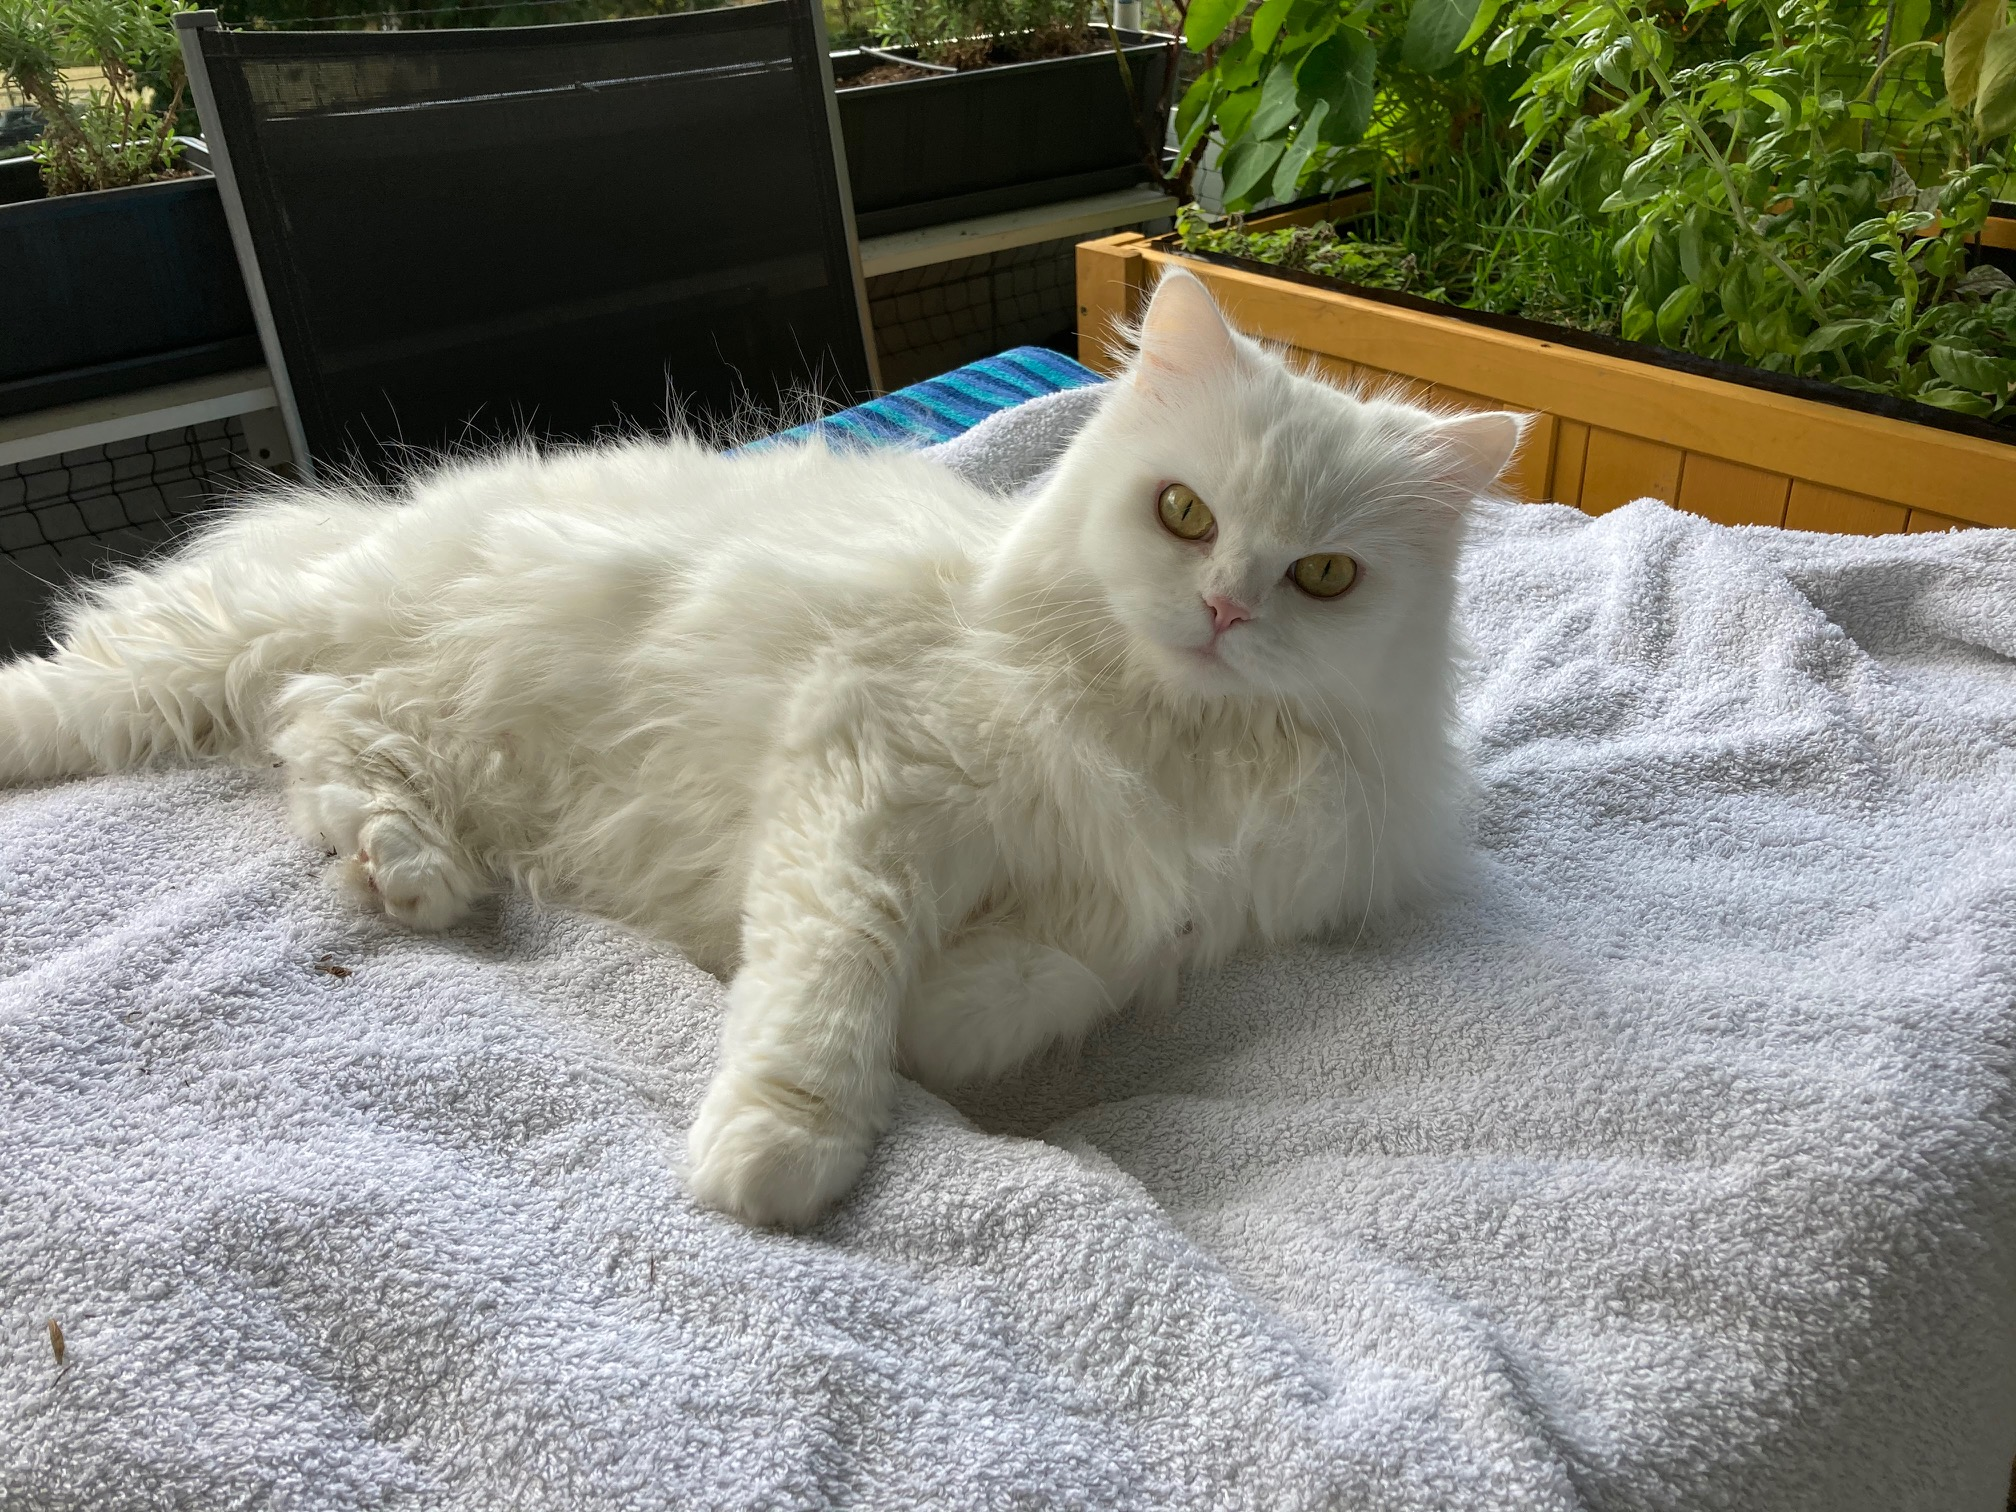
\includegraphics[width=0.2\textwidth]{Bilder/Katze1}
\end{center}

\vfill
Uwe Ziegenhagen \\
Matrikelnummer 31415927 \\
Köln, den \today 
\end{titlepage}

\tableofcontents
\listoffigures
\listoftables
	
\chapter{Einführung in das Thema}	
\section{Literaturüberblick}

In diesem Abschnitt wollen wir kurz die aktuelle Literatur zum Thema besprechen.	
	
\blindtext[10]

\begin{figure}
	\centering
	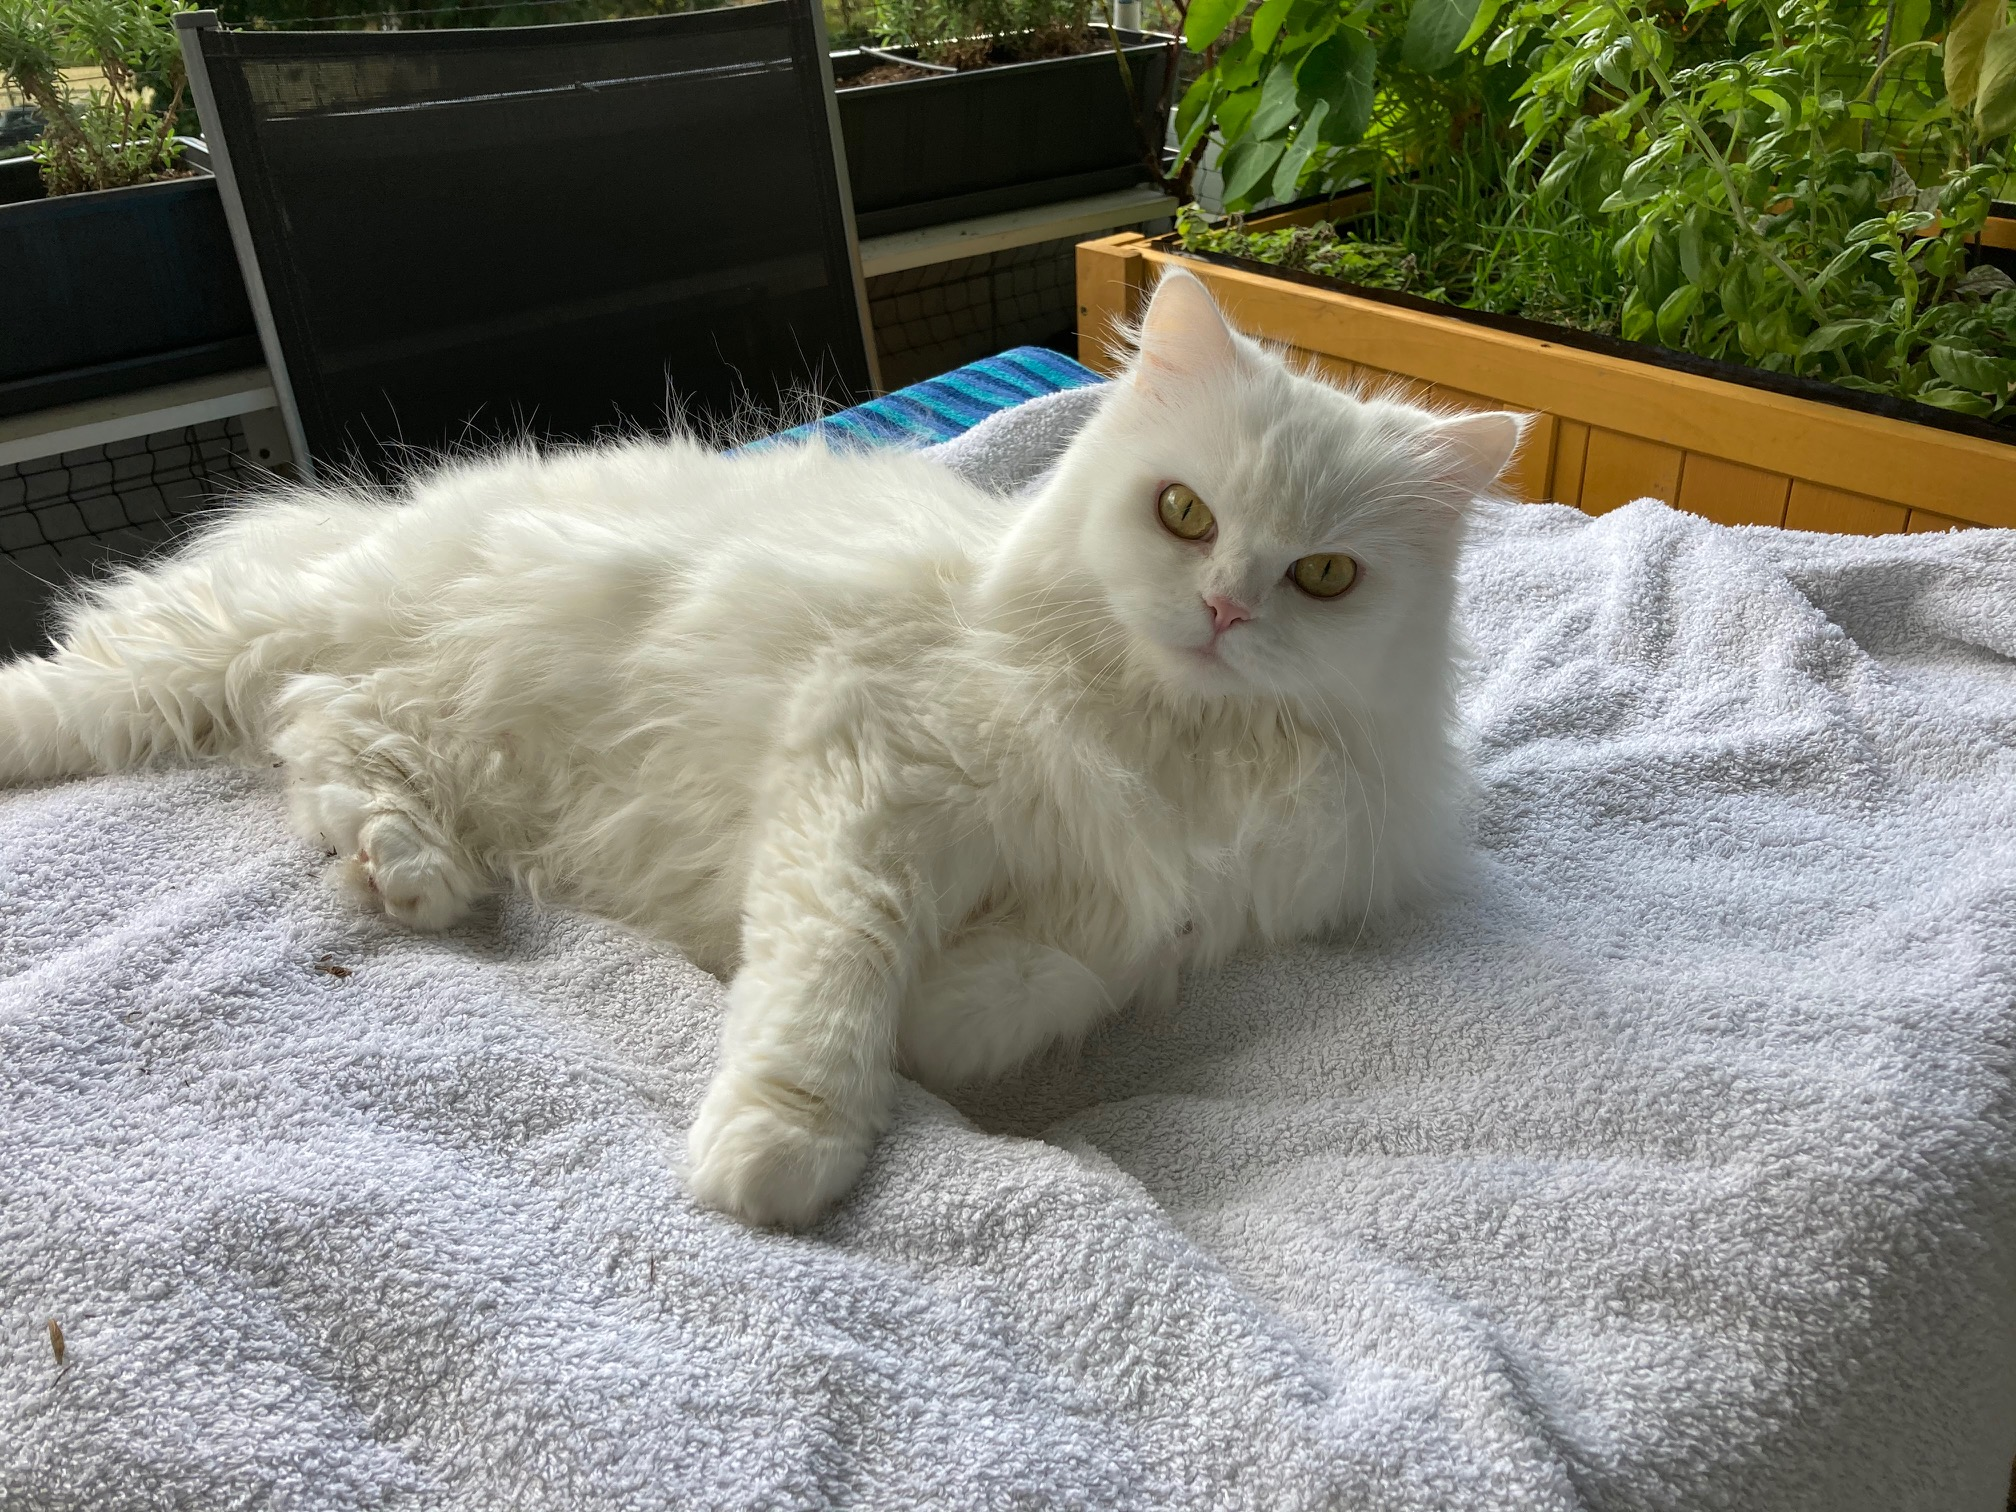
\includegraphics[width=0.75\textwidth]{Bilder/Katze1}
	\caption{Eine Miezekatze}\label{fig:katze1}
\end{figure}

\blindtext[10]
	
\end{document}

